% =====================================================================
% 3 METHODS
% src: analysis/cells.csv (provenance, h1x_*, ext_*, dev_* columns), /data/heretic_2/results/heretic/*/result.json and
%      study/*.jsonl, /data/heretic_2/paper32/configs/heretic_{general,code_specific}.toml, paper-33 configs/core_*.toml,
%      paper-33 scripts/bench/refusal_sets.json, paper-33 Methods (harness, judges, benchmarks).
% Revised 2026-11-06 (internal review): 1.x marker count 32 (not 33) and system prompt "You are a helpful coding
%   assistant." verified in all 12 Qwen2.5 study/*.jsonl settings records (results/heretic/Qwen__Qwen2.5-*/study);
%   2.0: 33 markers ("disclaimer" added; heretic src/heretic/scorers/keyword_rate.py @ 0db5c31) and system prompt
%   "You are a helpful assistant." (config.default.toml @ 0db5c31); 2.0 KL scorer has no target
%   (src/heretic/scorers/kl_divergence.py). 1.x selection rule from paper32/scripts/heretic_batch.py (--kl-max 0.01
%   default; result.json rule "min_refusals|kl<=0.01"). SOM / J-space: fork paper33-plugins @ 8fd4d76 (paper 33
%   08b_setup_details.tex). External tools: /data/heretic_2/tools_ext/README.md.
%   32B original harness: paper-33 runs/mc-rtx-1/results/bench/qwen2.5-32b__base/{summary.json, refusal_run/summary.json}
%   (no "postprocess" key) vs all other 32B cells ("U+2581 -> space"); paper-33 t2/t3 captions (bench.py revisions).
% Revised 2026-11-06 (pm, after assemble_p30.py re-run 22:47Z): all 7B 1.x cells judged; selection-cap re-export
%   (reexport_1x/VERSION.md, results_rtx/*/PROVENANCE.json, results_rtx/reexport_1x.log); external tools
%   (/data/heretic_2/models/external/*/PROVENANCE.json; cells.csv ext_*); Holm families from tests_refusal.csv
%   (column family, n_in_family) and tests_capability.csv (column family).
% Revised 2026-11-08 (ARS review): R12 search ranges and objectives of both builds in tab:h1setup (src:
%   analysis/revision_20261108/search_space.csv, read from the Optuna journals; identical to `git show
%   v1.4.0:src/heretic/main.py` l.566-601 and `git show 0db5c31:src/heretic/modifiers/abliteration.py` l.247-297 in
%   /data/heretic_2/heretic; 1.x objective: v1.4.0 evaluator.py get_score l.110-125); "same edit" -> "same edit family";
%   S11 Heretic DiM vs Arditi et al.; S20 fork identity (`git diff --stat 0db5c31 8fd4d76`: config.default.toml +63
%   lines, no deletions; new files modifiers/precomputed.py, modifiers/som.py, tests/test_som.py); R8 search-level
%   decision rule; S7 clustered correlations; S8 equivalence margin; S9 external contrasts descriptive; R5 "earlier
%   draft" removed; R11 "KL-matched" -> "rule-matched".
% =====================================================================
\section{Methods}
\label{sec:methods}

% 2026-11-07: study-design schematic (figures/src/gen.py, diagram-design primitives)
\begin{figure*}[tbp]
\centering
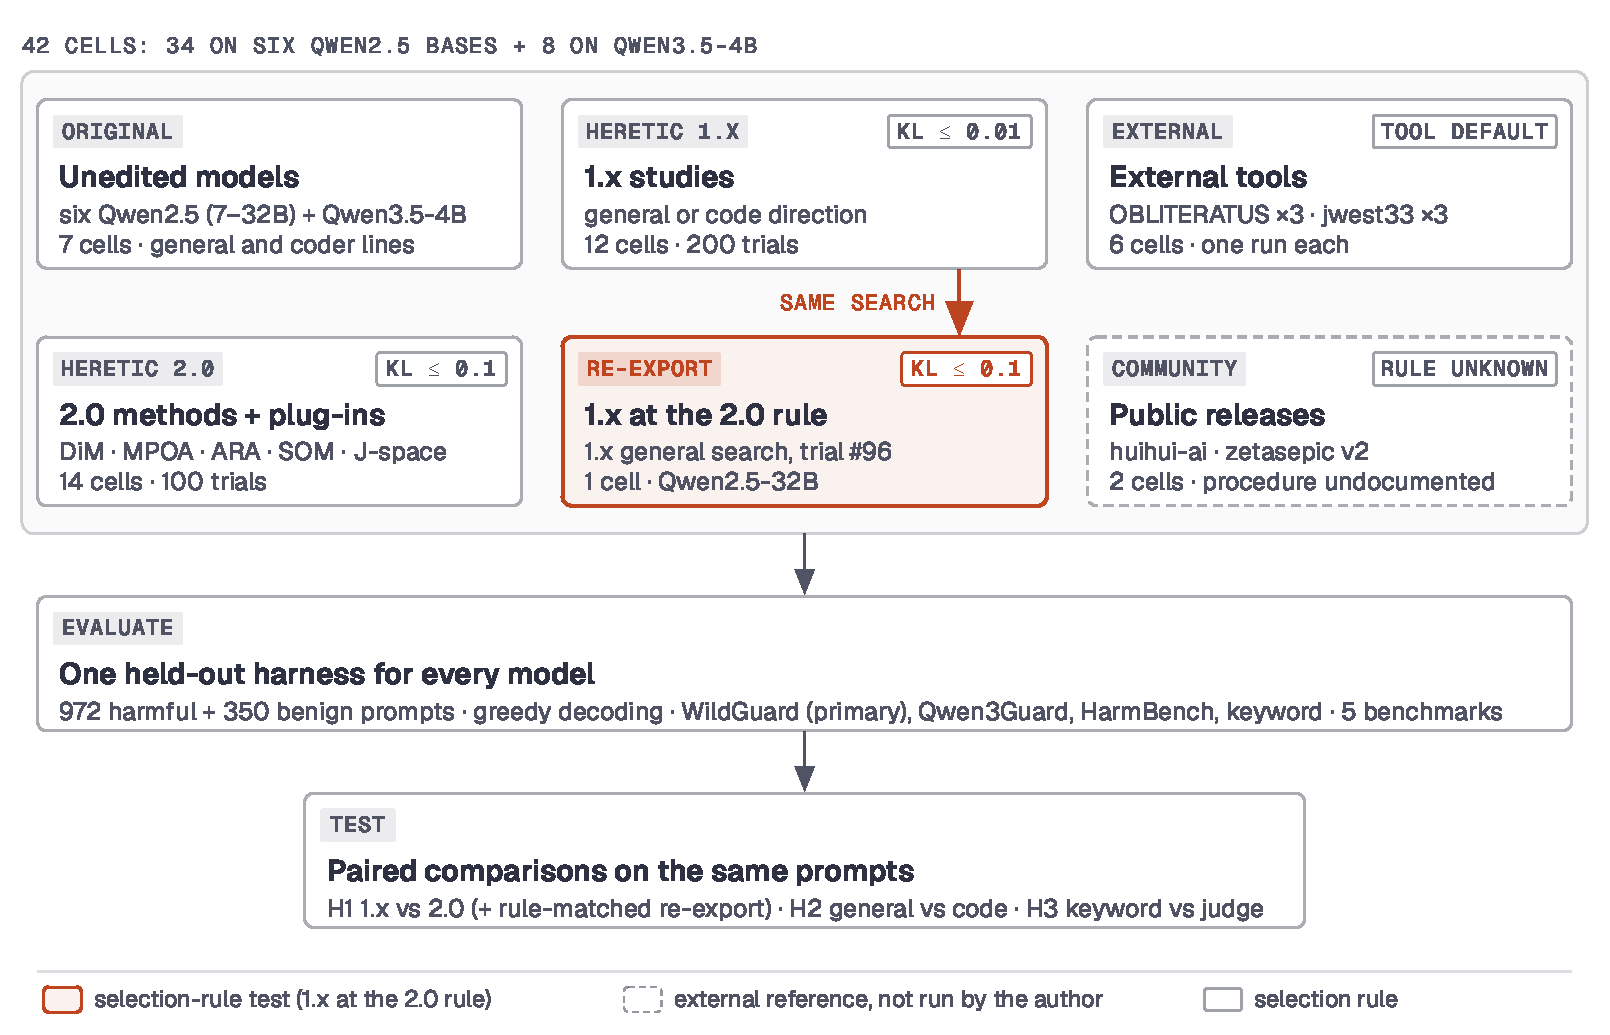
\includegraphics[width=\textwidth]{figures/fig0_study_design.pdf}
\caption{\textbf{Study design.} Six kinds of model on the same Qwen2.5 bases are evaluated with one held-out,
judge-based harness and compared with paired tests on the same prompts. The highlighted condition is the selection-cap
test: the original Heretic~1.x general study on Qwen2.5-32B re-exported at the Heretic~2.0 selection rule
(\S\ref{sec:reexport}). Community releases (dashed) were produced by others with undocumented procedures; the
external tools were run by the author with their default or recommended settings. ``Rule-matched'': both arms selected
by the same rule, not at matched divergence.}
\label{fig:design}
\end{figure*}

\subsection{Models and Conditions}
\label{sec:models}

% src (RESULTS.md "Coverage": 42 of 42 judged; scripts/supp_stats.py COMPANION set; cells.csv provenance)
All base models of the main design are Qwen2.5 instruction-tuned checkpoints \cite{qwen2024qwen25,hui2024qwen25coder}
in two lines, general (Qwen2.5-7B, -14B and -32B-Instruct) and coder (Qwen2.5-Coder-7B, -14B and -32B-Instruct), run
unquantised in bf16. Each base model is evaluated unedited (the \emph{original}) and after one or more edits
(Table~\ref{tab:conditions}, Figure~\ref{fig:design}); a model--condition combination is called a \emph{cell}. The main design has 29 cells,
all judged: the six originals, twelve Heretic~1.x models (a general and a code variant on each base model), nine
Heretic~2.0 and fork-plug-in models (five on Qwen2.5-7B, four on Qwen2.5-32B) and two community releases of
Qwen2.5-32B. Thirteen of these cells were first reported in the companion study \cite{young2026harder}: the
Qwen2.5-7B and Qwen2.5-32B originals, the nine Heretic~2.0 and fork-plug-in models and the two community releases.
Their responses and judge labels are reused here and are marked in the Source column of Table~\ref{tab:cells}. The
other 16 cells are new: the twelve 1.x models and the Qwen2.5-Coder-7B, Qwen2.5-14B, Qwen2.5-Coder-14B and
Qwen2.5-Coder-32B originals. Thirteen cells were added after the main design (\S\ref{sec:deviations}): the
Qwen2.5-32B 1.x general search re-exported at the Heretic~2.0 selection rule (\S\ref{sec:reexport}); four
external-tool cells on Qwen2.5-7B and two on Qwen3.5-4B (\S\ref{sec:external}); and, as context for the latter, the
Qwen3.5-4B original and its five seed-1 Heretic~2.0 and fork-plug-in models from the companion study, whose
responses and judge labels are reused. In total 42 cells were judged.

\begin{table*}[tbp]
\centering\small
\caption{Conditions. All Heretic edits act on the attention output projection and the MLP down-projection of each
layer. TPE = multivariate tree-structured Parzen estimator in Optuna; KL = first-token KL divergence from the
original on 100 harmless prompts (\texttt{mlabonne/harmless\_alpaca} test[:100]; 1.x code: its own benign-code
evaluation prompts); dev = development prompts whose
keyword refusals the search minimises. General direction data: \texttt{mlabonne/harmful\_behaviors} versus
\texttt{mlabonne/harmless\_alpaca}, train[:400] each; general dev set: \texttt{harmful\_behaviors} test[:100].
Fork plug-in: method from the project fork \texttt{paper33-plugins} (commit \texttt{8fd4d76}) of the companion
study, not part of the Heretic~2.0 releases. Heretic~1.x general and Heretic~2.0 DiM apply the same edit family
with different search ranges and objectives (Table~\ref{tab:h1setup}). Qwen3.5-4B cells of the 2.0 and fork configurations are seed-1 models of the companion
study, included as context for the external tools. External tools were run once at their own default or recommended
settings, without a search or a selection rule by the author (\S\ref{sec:external}).}
\label{tab:conditions}
\setlength{\tabcolsep}{4pt}
\begin{tabular}{@{}>{\raggedright\arraybackslash}p{2.25cm}>{\raggedright\arraybackslash}p{2.9cm}%
>{\raggedright\arraybackslash}p{2.75cm}>{\raggedright\arraybackslash}p{2.7cm}%
>{\raggedright\arraybackslash}p{2.55cm}>{\raggedright\arraybackslash}p{1.45cm}@{}}
\toprule
Condition & Edit & Direction data; dev set & Build and search & Selection rule & Models \\
\midrule
1.x general & rank-1 directional ablation, per-layer kernel; no projection, no row normalisation & general;
general & heretic-llm 1.4.0; TPE, 200 trials (60 random), seed~0 & fewest dev refusals at KL $\le$ 0.01 (archived
runs) & all six \\
1.x code & as 1.x general & malicious- vs benign-code prompts; 100 held-out malicious-code prompts & as 1.x general &
as 1.x general & all six \\
1.x general, KL $\le$ 0.1 & as 1.x general & as 1.x general & re-export of the archived 1.x general search
(\S\ref{sec:reexport}) & fewest dev refusals at KL $\le$ 0.1 (2.0 rule): trial \#96 & 32B \\
\midrule
2.0 DiM & rank-1 DiM ablation (same edit family as 1.x) & general; general & Heretic~2.0.0; TPE, 100 trials (30 random),
seed~1 & fewest dev refusals at KL $\le$ 0.1 (companion study) & 7B, 32B; Qwen3.5-4B \\
2.0 MPOA & projected, norm-preserving (rank 3) & as 2.0 DiM & as 2.0 DiM & as 2.0 DiM & 7B, 32B; Qwen3.5-4B \\
2.0 ARA & rank-50 LoRA per module, L-BFGS & as 2.0 DiM & as 2.0 DiM & as 2.0 DiM & 7B, 32B; Qwen3.5-4B \\
SOM (fork plug-in) & $k=4$ SOM directions, projected, norm-preserving (rank 6) & as 2.0 DiM & fork \texttt{8fd4d76}; as 2.0
DiM & as 2.0 DiM & 7B, 32B; Qwen3.5-4B \\
J-space (fork plug-in) & Jacobian-lens direction, row-normalised (rank 3) & lens direction (no contrast set);
general & fork \texttt{8fd4d76}; as 2.0 DiM & as 2.0 DiM & 7B; Qwen3.5-4B \\
\midrule
Community & not documented & -- & -- & -- & 32B \\
\midrule
OBLITERATUS: \texttt{basic}, \texttt{advanced}, \texttt{spectral\_}\allowbreak\texttt{cascade} & tool presets (\S\ref{sec:external}) &
tool's built-in 842 harmful and 842 harmless prompts & v0.1.4 (\texttt{461ff086}); preset defaults, seed~1 & none
(tool output) & 7B \\
jwest33 abliterator & all linear layers; norm-preserving, winsorised, null-space constrained & 30 harmful and 30
harmless prompts sampled from the tool's pools & commit \texttt{6ca3356e}; recommended settings, seed~1 & none
(tool output) & 7B; Qwen3.5-4B (as released; hybrid fix as sensitivity run) \\
\bottomrule
\end{tabular}
\end{table*}

% src (reexport_1x/VERSION.md: heretic-llm 1.4.0 = git v1.4.0 6ea3b8d, evidence 1-5; cells.csv adapter_sha256_ok,
%      tensors_*; reexport_1x/validation_7b/SUMMARY.json for the 7B general merge check; code-study journals
%      results/heretic/Qwen__*__code/study/*.jsonl: trial user attr n_bad_prompts = 100 in all six studies (1.4.0
%      main.py l.644: len(evaluator.bad_prompts), evaluator.py l.38: bad_evaluation_prompts); settings
%      good/bad(_evaluation)_prompts = configs/code_abliteration_data/{benign_code_prompts,malicious_code_prompts,
%      benign_code_eval,malicious_code_eval}.txt)
\paragraph{Heretic~1.x.} Rank-1 LoRA adapters \cite{hu2022lora} produced in June 2026 with Heretic~1.x
\cite{heretic2025} were available for all six base models in two variants; they were produced by the author's earlier, unpublished
code-abliteration study. The run records do not name the release,
but the key set and order of the settings record stored in every 1.x study journal, together with the search range
that the journals record for the MLP ablation weight, identify it as heretic-llm 1.4.0 (git tag \texttt{v1.4.0},
commit \texttt{6ea3b8d}); earlier revisions store a different key order and later ones a different search range
(Appendix~\ref{app:reexport}). The \emph{general} variant computes the refusal direction from the first 400
training prompts of \texttt{mlabonne/harmful\_behaviors} and \texttt{mlabonne/harmless\_alpaca}
\cite{zou2023universal,taori2023alpaca}, as Heretic does by default. The \emph{code} variant computes it from
malicious-code requests (RMCBench and MalwareBench) against benign coding prompts (MBPP), uses a held-out file of
malicious-code requests as its dev set (100 prompts, the count stored with every trial) and a file of benign coding
prompts for its KL term. The code pipeline therefore differs from the general one in its direction data, dev set
and KL prompts, not only in its direction. These four prompt files, and the script that generated them, were not archived with the
run records, so their contents and the sizes of the direction sets are unknown. Both variants ran 200 TPE trials (60 random) with
seed~0, the optimisation system prompt ``You are a helpful coding assistant.'', at most 100 generated tokens per dev
response, a list of 32 keyword markers (Heretic's default list without ``disclaimer''), and a KL target of 0.01:
the 1.x objective is a pair of minimised scores, the KL divergence (replaced, below the target, by the normalised
refusal count times the target) and the refusal count normalised by the base model's dev refusals. The 1.x build also exposed the
direction-projection and row-normalisation options that define MPOA, but the archived runs switched them off. The
released trial was chosen by the archived study's batch wrapper, not by Heretic: the fewest dev refusals among trials
with KL $\le$ 0.01, a cap met in all 12 runs. Each adapter was merged into its base model on CPU. The SHA-256 of all
12 adapters matched their manifests; for the eight 14B and 32B adapters the rebuilt merges were tensor-for-tensor
identical to the archived merges, and for the four 7B adapters no tensor hashes of the archived merges had been
recorded (Appendix~\ref{app:checks}).

Heretic's directional ablation, in both versions, differs from the edit of Arditi et al.\ \cite{arditi2024refusal},
which orthogonalises every residual writer, including the embedding, against one direction at full strength: Heretic
edits only the attention output and MLP down-projections, with a per-layer weight kernel (a maximum weight, its
position and a minimum weight at a given distance) and either one direction interpolated between two layers'
directions or a separate direction per layer, all chosen by the search.

\paragraph{Heretic~2.0 and fork plug-ins.} The Heretic~2.0 models are the seed-1 models of the companion study
\cite{young2026harder}: DiM (a difference-in-means direction \cite{arditi2024refusal} applied with Heretic's
per-layer weight kernel), MPOA \cite{lai2024projected,lai2025mpoa} and ARA
\cite{weidmann2026ara}, which are built into Heretic~2.0.0 (upstream commit \texttt{0db5c31}), on Qwen2.5-32B and
Qwen2.5-7B. SOM \cite{piras2025som} (on both models) and J-space ablation \cite{sekinal2026jspace} (on Qwen2.5-7B
only) are plug-ins of the companion study's project fork (branch \texttt{paper33-plugins}, commit \texttt{8fd4d76});
they are not part of any Heretic~2.0 release. SOM ports the proof of concept of Heretic pull request~\#196, and
J-space bakes directions from the \texttt{jspace-refusal} code into the weights with Heretic's row-normalised
directional ablation instead of the reference forward hook. All Qwen2.5-7B runs, including DiM, MPOA and ARA, ran
from the fork; \texttt{git diff 0db5c31 8fd4d76} shows that the fork only adds files (the SOM and
precomputed-direction modifiers and their tests) and configuration entries, without changing any line of an existing
source file, so the built-in methods are identical to \texttt{0db5c31}. All used the general direction data
and dev set, 100 TPE trials (30 random) with seed~1, Heretic~2.0's default system prompt ``You are a helpful
assistant.'', its 33 default keyword markers (the 1.x list plus ``disclaimer''), KL as a plain minimised objective,
and the companion study's selection rule: the fewest dev refusals among trials with KL $\le$ 0.1, ties broken by
lower KL. The companion study's seed-1 models of the same five configurations on Qwen3.5-4B serve only as context
for the external-tool cells on that model; they enter no test of H1--H3.

% src (tab:h1setup rows: cells.csv dev_refusals/dev_kl; RESULTS.md "Dev set at matched KL caps": 1x_general 32B
%      <=0.1 -> 50 (0.064); dim 32B selected 89 @ 0.0175; 2026-11-08 search-range and selected-weight rows:
%      analysis/revision_20261108/search_space.csv (journal distributions; selected_value of mlp.down_proj.max_weight:
%      32B #84 0.9115, #96 1.0019, DiM #62 1.2133; 7B #193 1.1455, DiM #36 1.1863))
\begin{table}[tbp]
\centering\small
\caption{Setup of the like-for-like contrast (H1). Both arms apply the same edit family with the same direction
data, dev prompts and KL prompts. Search ranges are those recorded in each search's Optuna journal ($L$ = index of
the last layer; 63 for Qwen2.5-32B, 27 for Qwen2.5-7B); they agree with the source of heretic-llm~1.4.0 and of
Heretic \texttt{0db5c31}. The only range that differs is that of the MLP maximum weight; no selected or re-exported
trial used a value below 0.8. Released trial: dev keyword refusals of 100 (dev KL), each counted under its own arm's
system prompt and marker list. The last row gives the trial that the 2.0 rule selects from each search on
Qwen2.5-32B; the 1.x trial was re-exported and evaluated (\S\ref{sec:reexport}).}
\label{tab:h1setup}
\setlength{\tabcolsep}{4pt}
\begin{tabular}{@{}>{\raggedright\arraybackslash}p{3.0cm}>{\raggedright\arraybackslash}p{5.2cm}%
>{\raggedright\arraybackslash}p{5.2cm}@{}}
\toprule
Setting & Heretic~1.x general (archived runs) & Heretic~2.0 DiM (companion study) \\
\midrule
Edit & rank-1 directional ablation, no projection, no row normalisation & same \\
Direction & global (interpolated) or per layer; index in $[0.4L, 0.9L]$ & same \\
Attention max.\ weight & $[0.8, 1.5]$ & same \\
MLP max.\ weight & $[0.8, 1.5]$ & $[-0.25, 1.5]$, clamped at 0 \\
Weight kernel & position $[0.6L, L]$; min.\ weight $[0, 1]\times$max.; distance $[1, 0.6L]$ & same \\
Selected MLP max.\ weight & 32B: 0.91 (\#84), 1.00 (\#96); 7B: 1.15 & 32B: 1.21; 7B: 1.19 \\
Direction data; dev; KL prompts & general; general; \texttt{harmless\_alpaca} test[:100] & same \\
Build & heretic-llm 1.4.0 (\texttt{6ea3b8d}) & v2.0.0 (\texttt{0db5c31}); Qwen2.5-7B: fork
\texttt{8fd4d76} \\
Trials (random), seed & 200 (60), seed~0 & 100 (30), seed~1 \\
Optimisation system prompt & ``You are a helpful coding assistant.'' & ``You are a helpful assistant.'' \\
Keyword markers (dev) & 32 & 33 (adds ``disclaimer'') \\
Objective (both minimised) & KL with target 0.01 (below it: scaled refusal score); refusals / base refusals &
keyword refusal rate; KL, no target \\
Selection rule & fewest dev refusals, KL $\le$ 0.01 & fewest dev refusals, KL $\le$ 0.1 \\
Released trial, Qwen2.5-32B & 89 (0.006) & 89 (0.018) \\
Released trial, Qwen2.5-7B & 67 (0.005) & 55 (0.078) \\
Trial at the 2.0 rule, Qwen2.5-32B & 50 (0.064), trial \#96, re-exported & 89 (0.018), the released trial \\
\bottomrule
\end{tabular}
\end{table}

\paragraph{Community releases.} Two public abliterations of Qwen2.5-32B-Instruct were evaluated as released:
\path{huihui-ai/Qwen2.5-32B-Instruct-abliterated} (revision \texttt{546fc405}) \cite{huihui2025qwen32b} and
\path{zetasepic/Qwen2.5-32B-Instruct-abliterated-v2} (revision \texttt{5894fbf0}) \cite{zetasepic2025qwen32b}.
Their procedures, prompt sets and selection rules are not documented.

\subsection{Selection-Cap Re-Export}
\label{sec:reexport}

% src (reexport_1x/VERSION.md; reexport_1x/run_on_rtx.sh header (rule: KL <= 0.1, fewest dev refusals, ties -> lower
%      KL; general #96 50/100 KL 0.0642, code #134 2/100 KL 0.0717); results_rtx/qwen2.5-32b__heretic1x-general-kl0.1/
%      PROVENANCE.json (journal_sha256 bf60f054..., settings_roundtrip_identical, base_model_revision 5ede1c97,
%      journal_values 50 @ 0.06423, reevaluated 51 @ 0.06367, n_edited_modules 80, verdict PASS);
%      results_rtx/trial84_validation_records/PROVENANCE.json (validation.adapter: 62/62, min_direction_cosine
%      0.9999876; reevaluated 90 @ 0.00553; reevaluated_original_adapter_here 90 @ 0.00535; journal 89 @ 0.00592);
%      results_rtx/reexport_1x.log l.246-248 (merged 709/771 identical, max_abs_diff 0.0078125, PASS))
The two arms of the like-for-like contrast were released under different selection caps (dev KL $\le$ 0.01 for
1.x, $\le$ 0.1 for 2.0). To separate the cap from the version, the archived Heretic~1.x general search on
Qwen2.5-32B was re-exported at the 2.0 rule. The re-export used heretic-llm 1.4.0 with the dependency versions
locked by that release (transformers 5.6.2, PEFT 0.19.1, Optuna 4.8.0) and PyTorch 2.14.1, because the PyTorch
version of the original runs was not recorded. A re-export script loaded the original study journal, checked that its stored
settings pass unchanged through the 1.4.0 settings class (only the local model path and the automatic batch size
were overridden), recomputed the refusal directions with the 1.4.0 code from the same prompts, rebuilt the rank-1
adapter of the requested trial from its stored parameters, re-evaluated it on the 100 dev and 100 KL prompts and
merged it into the base model (revision \texttt{5ede1c97}). The trial selected by the 2.0 rule (fewest dev
refusals among trials with dev KL $\le$ 0.1, ties broken by lower KL) was trial~\#96: 50 of 100 dev refusals at a
dev KL of 0.064 in the journal, and 51 at 0.064 on re-evaluation. The released trial~\#84 had 89 at 0.006.

Before trial~\#96 was used, the same script re-exported the released trial~\#84 and compared it with the archived
adapter; a failure of this gate would have stopped the run before trial~\#96 was exported. The re-exported and
archived adapters edited the same 62 modules; their weights were not bit-identical, but the minimum direction cosine
between corresponding modules was 0.99999. In the merged models 709 of 771 tensors were bit-identical, and the other
62 differed by at most 0.0078 in absolute value. The re-exported adapter kept 90 dev refusals, the archived adapter
evaluated in the same run 90 and the journal 89. The re-export was therefore accepted as numerically equivalent to the
original, and the trial~\#96 model was evaluated with the same harness as every other cell. The 1.x code search could
not be re-exported, because its four prompt files (the malicious- and benign-code direction prompts and the two
evaluation files) were never copied from the archived study's repository; without them its refusal directions cannot
be recomputed. Only the general variant on Qwen2.5-32B therefore has a KL $\le$ 0.1 cell. Provenance and the
acceptance criteria are given in Appendix~\ref{app:reexport}.

\subsection{External Tools}
\label{sec:external}

% src (/data/heretic_2/models/external/*/PROVENANCE.json: commit, preset, preset_definition, resolved_config,
%      runtime_patches, hybrid_detection, seed, base_revision, prompt_sets, tool_reported_metrics; cells.csv ext_*;
%      tools_ext/README.md (preset mapping, som not shipped, Qwen3.5 contract, CLI hybrid-detection omission))
Two external abliteration tools were run by the author with each tool's documented default or recommended settings
and evaluated with the same harness as the Heretic cells. No search over their settings was made and their outputs
were not selected by dev KL; each tool contributes the single model it produced. Every run used seed~1, bf16 weights
and the base revisions of the Heretic cells (Qwen2.5-7B-Instruct \texttt{a09a3545}, Qwen3.5-4B \texttt{851bf6e8}).
The tools' code was used from clean checkouts; every deviation is a named runtime patch in a wrapper, recorded in
each output's provenance record (Appendix~\ref{app:external}).

OBLITERATUS \cite{obliteratus2026} v0.1.4 (commit \texttt{461ff086}) was run with three presets on Qwen2.5-7B,
\texttt{basic}, \texttt{advanced} and \texttt{spectral\_cascade}, through the tool's Python pipeline with every
preset default (bf16 instead of the command-line default float16) and no runtime patch. All presets compute
directions from the tool's built-in list of 842 harmful and 842 harmless prompts, of which one harmful prompt is a
held-out JailbreakBench prompt that also belongs to the 44 AdvBench-overlap prompts (\S\ref{sec:measures}).
\texttt{basic} is the preset closest to Arditi et al.\ (one difference-in-means direction, no norm preservation),
but it is not a reproduction of that method or of Heretic's DiM: it feeds the prompts without the chat template and
edits only the layers chosen by its knee-based heuristic (ten layers on Qwen2.5-7B), whereas Arditi et al.\
orthogonalise every residual writer. \texttt{advanced} removes four SVD directions with norm preservation and
regularisation (seven layers); \texttt{spectral\_cascade} removes six whitened-SVD directions, extracted with an
additional jailbreak contrast, with iterative refinement and a frequency decomposition of the refusal signal across
layers (16 layers). The \texttt{som} preset is listed in v0.1.4 but its
direction module is not shipped, so the preset fails by design and is reported as not available. OBLITERATUS v0.1.4
does not support Qwen3.5-4B: for the hybrid-attention Qwen3.5 architecture its validation step accepts only one
larger Qwen model and stops before any weight is modified, so no OBLITERATUS model exists for Qwen3.5-4B and that
cell is reported as not supported.

The jwest33 abliterator \cite{jwest33abliterator} (commit \texttt{6ca3356e}) was run through its own batch command
line with the settings that its interactive mode labels as recommended (``Recommended standard'' for dense models,
``Recommended for hybrid model'' for Qwen3.5; both translate to the same batch flags): winsorisation and the
null-space constraint, with norm preservation, projected refusal directions, all linear layers of the language model
and the other values at their defaults. The tool samples 30 harmful and 30 harmless prompts from its default pools
(5{,}000 each) and filters the harmful ones by a log-likelihood refusal test. Three wrapper measures leave the
tool's code unchanged: the prompt files, deleted from the repository after commit \texttt{a2a7940}, are supplied
from that commit; the tool's unseeded prompt sampling is seeded; and the prompts actually used are recorded. All
three jwest33 runs used the same 30 harmful and 30 harmless prompts. One of the harmful prompts is a held-out
JailbreakBench prompt that also belongs to the 44 AdvBench-overlap prompts, so the analysis without those prompts
excludes it. The tool's known behaviour on square residual writers, which it projects on the input side (the
$3{,}584\times3{,}584$ attention output projection of Qwen2.5-7B), was left uncorrected.

The tool's library entry point detects hybrid architectures and, for them, restricts direction extraction to the
full-attention layers and the linear-attention layer before each and down-weights the linear-attention layers; its
batch command line omits that detection, so the documented default hybrid strategy has no effect there. On
Qwen3.5-4B the primary cell is the tool as released (no runtime patch). A second run with a runtime patch that sets
the detected architecture information before direction extraction, as the library entry point does, is reported as
a sensitivity analysis; the as-released run was designated primary before it was generated. On Qwen2.5-7B, which the
tool detects as non-hybrid, the same patch was active but changes nothing, so the Qwen2.5-7B cell is in effect the
tool as released. The Qwen3.5-4B cells lie outside the Qwen2.5 design; they are compared with the Qwen3.5-4B
original and its five companion-study models (\S\ref{sec:models}).

% src (PROVENANCE.json tool_reported_metrics: OBLITERATUS refusal_rate 0.833/0.400/0.033, verify_sample_size 30;
%      jwest33: filter settings only; assemble_p30.py l.553-554)
Both tools check their output on their own prompts. OBLITERATUS reports a refusal rate on a verification sample of 30
prompts from its built-in harmful list, together with perplexity, coherence and a sequence-level KL divergence;
jwest33's batch run reports its filter settings but no refusal rate. These self-reports use other prompts, markers
and generation lengths than the held-out harness and are not comparable with its measures; the OBLITERATUS refusal
rate is used only to check whether the tool's own assessment agrees in direction with the judged result.

\subsection{Measures}
\label{sec:measures}

% src (RESULTS.md "Coverage" WG N/A column and "Anomalies and checks": 2 harmful (qwen2.5-32b__base,
%      qwen2.5-7b__obliteratus-advanced), 1 benign (qwen2.5-7b__som) of 42 x 972 = 40,824 / 42 x 350 = 14,700;
%      judge revisions; degenerate() in paper-33 scripts/bench/score_refusals.py)
\paragraph{Held-out refusal.} One greedy response (at most 512 new tokens, the model's chat template, system
prompt ``You are a helpful assistant.'') to each of 1{,}322 held-out prompts was generated with vLLM
\cite{kwon2023efficient}. The 972 harmful prompts comprise JailbreakBench harmful (100), XSTest unsafe (200),
StrongREJECT (313), HarmBench standard (159) and a code-as-weapon sample (200; malicious-code requests whose
answer would be working attack code)
\cite{chao2024jailbreakbench,rottger2024xstest,souly2024strongreject,mazeika2024harmbench,young2026code}; the 350
benign prompts are JailbreakBench benign (100) and XSTest safe (250). The set is held out from search and selection
except for 44 harmful prompts that exactly (36) or approximately (8) match a prompt of \texttt{harmful\_behaviors},
which are analysed with and without; 41 code-as-weapon prompts come from RMCBench or MalwareBench, the sources of
the 1.x code direction, and are likewise analysed with and without for H2. The \emph{primary outcome} is the
WildGuard \cite{han2024wildguard} refusal label of each harmful response (residual refusal); responses without a
WildGuard label (2 of 40{,}824 harmful and 1 of 14{,}700 benign responses) are dropped pairwise. Secondary refusal
measures are Heretic~2.0's 33 default keyword markers on the full response and on its first 256 tokens, and the
refusal label of Qwen3Guard-Gen-8B \cite{zhao2025qwen3guard}; harmful compliance is the HarmBench classifier's label
\cite{mazeika2024harmbench}; over-refusal is the WildGuard refusal rate on the benign prompts. A response that reached
the 512-token limit is called \emph{capped}. A response is flagged \emph{degenerate} by the harness's heuristic
\cite{young2026harder} if it is empty, if more than half of its word 4-grams repeat or fewer than 15\% of its words
are distinct (responses of at least 20 words), if it contains a run of more than 40 identical characters (code and
markdown separators excepted) or if more than 20\% of its characters are non-printable; degenerate responses keep
their judge labels and are reported as a rate. Judge revisions were identical for every cell (WildGuard
\texttt{cbba4823}, Qwen3Guard \texttt{4505cb1a}, HarmBench classifier \texttt{bda70534}).

\paragraph{Capability and distribution shift.} Five benchmarks ran with lm-evaluation-harness 0.4.13
\cite{gao2024language} on vLLM 0.33.0 with greedy decoding: MMLU-Pro (1{,}000 items) \cite{wang2024mmlupro},
GSM8K (500) \cite{cobbe2021training}, IFEval (541) \cite{zhou2023instruction}, HumanEval (164)
\cite{chen2021evaluating} and MBPP (500) \cite{austin2021program}. Distribution shift on held-out data is the
\emph{teacher-forced (TF) divergence}: the token-averaged $\log p_{\mathrm{orig}}(y)-\log p_{\mathrm{mod}}(y)$ over
the original model's own greedy responses $y$ to the 350 benign held-out prompts. The \emph{dev KL} is the
first-token KL divergence that the search recorded for a trial on its KL prompts (\texttt{harmless\_alpaca}
test[:100]; for the 1.x code variant, its own benign-code evaluation prompts). The \emph{selection
rule} picks the released trial from a search, its \emph{selection cap} is the dev-KL threshold of that rule, and
the \emph{search budget} is the number of trials. ``Divergence'' without qualification is not used for dev KL. The
external tools have no dev KL; the divergence figures they report themselves (Appendix~\ref{app:external}) are not
used in the analysis.

\subsection{Procedure}
\label{sec:procedure}

% src (cells.csv ref_dir/gen_dirs/cap_dir: results/bench-4090/* for the new 7B, Coder-7B and Qwen3.5-4B jwest33
%      cells; eval.log host=4090-omarchy, "NVIDIA GeForce RTX 4090"; summary.json judge_revisions;
%      runs/mc-rtx-1/results/bench/qwen2.5-32b__heretic1x-general-kl0.1; external PROVENANCE.json gpu RTX 4090;
%      reexport PROVENANCE.json environment.gpus RTX PRO 6000 Blackwell Server Edition)
% src (2026-11-08 re-review NEW-3): 33_.../runs/mc-h200-1/runs/qwen2.5-32b__{dim,mpoa,som,ara}__core-s1/meta.txt
%      ("torch 2.14.1+cu130 NVIDIA H200 NVL", heretic 0db5c31); revision_20261108/search_cost.csv (7B 2.0/fork searches
%      RTX 4090 from meta.txt; 1.x searches gpu "not recorded")
The 14B and 32B models, including the KL $\le$ 0.1 re-export, and the judges of all companion-study cells ran on one
NVIDIA RTX PRO 6000 (96 GB); the re-export itself was computed on an RTX PRO 6000 of the same type. The companion
study's Qwen2.5-7B and Qwen3.5-4B models were generated and benchmarked on an RTX 4090 and judged on the RTX PRO
6000. The new Qwen2.5-7B and Qwen2.5-Coder-7B cells (1.x and external tools) and the two jwest33 Qwen3.5-4B cells
were generated, benchmarked and judged on the RTX 4090 with the same judge revisions; the external tools also ran
there. The companion study's Heretic~2.0 and fork searches ran on one NVIDIA H200 NVL (Qwen2.5-32B) and on the
RTX 4090 (Qwen2.5-7B) \cite{young2026harder}; the GPUs of the archived 1.x searches were not recorded. Within each
base model, all cells used the same prompts, decoding settings, reference responses for TF
divergence and judges, with one exception. The Qwen2.5-32B original was evaluated in two earlier harness runs
(capability; held-out generation and teacher forcing) whose evaluation-script revision differs from that of its
edited models; these runs did not apply the output post-processing of later runs (mapping the SentencePiece
character U+2581 to a space; the original's outputs contain none), and its MBPP run predates the patched answer
extractor, so its per-item MBPP samples are unpatched and only its MBPP summary score was rescored from the logged
outputs \cite{young2026harder}. Data checks are listed in Appendix~\ref{app:checks}.

\subsection{Data Analysis}
\label{sec:stats}

% src (2026-11-08): sigma 9.15 [6.40, 16.07], SD_diff 12.95, threshold 25.89 [18.09, 45.44], equal-batch threshold 20.35:
%   analysis/revision_20261108/seednoise_derivation.csv (recomputed from paper-33 results/analysis/seednoise_seed_pairs.csv;
%   identical to paper-33 seednoise_sigma.csv and review_sel_seed_sigma.csv); equivalence margin and TOST:
%   revision_20261108/capability_equivalence.csv; clustered correlations: revision_20261108/correlations_clustered.csv.
% src (2026-11-08 re-review S7): revision_20261108/s7_correlations.csv (n_boot_degenerate 0 for all; within_model_p_scipy
%   0.0045 / 0.19 / 0.0026; within_model_p_df_adjusted 0.013 / 0.218 / 0.0088 for tf, dev_kl general, capability).
% src (tests_refusal.csv n_in_family by family: vs_base 23, h1_1x_vs_2.0 18, h2_general_vs_code 6,
%      within_model_pairs 76, kw_vs_judge 29; vs_base_added 12, h1_kl_matched 4, kl_cap_1x 1, external_vs_heretic 38,
%      external_sensitivity 1, kw_vs_judge_added 13; tests_capability.csv family original_design 23 cells x 5,
%      added 12 cells x 5; assemble_p30.py correlations(): original design only)
Rates carry Wilson 95\% intervals \cite{wilson1927probable}. Two models evaluated on the same prompts are compared
by the paired difference in rates with Newcombe's hybrid score interval \cite{newcombe1998improved} and the exact
McNemar test \cite{mcnemar1947note}, a prompt-level paired comparison \cite{miller2024adding}; each test therefore
compares two released checkpoints on these prompts and conditions on their searches. Holm's procedure
\cite{holm1979simple} controls each family of tests at two-sided $\alpha=0.05$, separately for each refusal measure
and prompt subset. The families of the main design are: each edited model versus its original (23 tests); the
1.x-versus-2.0 family, each 1.x variant versus each 2.0 method or fork plug-in on the same base model (18 tests, 8
on Qwen2.5-32B and 10 on Qwen2.5-7B); H2, 1.x general versus 1.x code per model (6 tests per subset); all pairs of
cells within a model (76 pairs, exploratory); and H3, keyword versus WildGuard on the same responses of each cell
(29 tests). The primary H1 test is the 1.x general versus 2.0 DiM contrast on each base model; it is adjusted within
the whole 1.x-versus-2.0 family, which is conservative for it, and the other contrasts of that family describe the
additional configurations. The added cells form separate families, so that the main-design results do not change
with their addition: each added cell versus its original (12 tests); the KL $\le$ 0.1 re-export versus the four
2.0 and fork configurations on Qwen2.5-32B (4 tests); the KL $\le$ 0.1 versus the KL $\le$ 0.01 export of the same
search (1 test, unadjusted); each external-tool cell versus each Heretic cell on the same base model (38 tests);
jwest33 as released versus with the hybrid fix (1 test, unadjusted); and keyword versus WildGuard for the added
cells (13 tests). Capability is compared per item with the same paired interval and test, Holm-adjusted over the
115 cell--benchmark tests of the main design and separately over the 60 of the added cells; the mean change over
the five benchmarks carries a normal interval from the per-benchmark paired variances. MBPP changes on the
Qwen2.5-32B original use an unpaired normal test on the summary scores (\S\ref{sec:procedure}). Whether a
capability change is negligible is assessed with two one-sided tests against an equivalence margin of $\pm$2~pp on the
mean of the five benchmarks (equivalence when the 90\% interval lies inside the margin); the margin was chosen after
the results were known, and the minimum change detectable with 80\% power is reported beside it. Associations across
edited models are Spearman correlations over the 23 edited models of the main design. Because these models are
clustered in six base models, their intervals come from a bootstrap that resamples base models with all their cells
(4{,}000 resamples, percentile intervals; a resample in which either variable was constant or fewer than four cells
remained would have been skipped, and none was), and each correlation is also reported for values centred within each
base model, the analogue of base-model fixed effects. The $p$-value of a within-base correlation is that of the
Spearman test on the centred values of the base models with at least two cells (t approximation with $n-2$ degrees of
freedom); it does not deduct the degrees of freedom used by centring and is therefore somewhat liberal (with that
deduction the within-base $p$-values of \S\ref{sec:res-tradeoff} become 0.013 for TF divergence, 0.22 for dev KL and 0.009 for capability). The original
percentile bootstrap over cells is kept in the analysis records. The association
with dev KL is reported only for the cells scored on the general dev protocol, because the code variants measure dev
KL on other prompts. All cross-model correlations are exploratory. Within a base model, the association of residual refusal with TF
divergence is a Spearman correlation with an exact permutation $p$-value. To separate search quality from the
selection rule, the fewest dev refusals reachable at dev-KL caps of 0.01 to 0.5 were read from the optimisation
records: the Pareto fronts of the 1.x runs and all trials of the 2.0 runs (the fewest refusals under a cap is always
attained on the Pareto front, so the two sources give the same values). The same records give each arm's fewest dev
refusals at the realised dev KL of the other arm's released trial, a comparison at matched dev divergence on the dev
prompts only.

\paragraph{Search-level decision rule.} The hypotheses concern versions, settings and pipelines, so their unit of
replication is the search, and each configuration contributed one search per base model. A prompt-level test
quantifies only prompt-sampling noise for two fixed checkpoints. Search-to-search variation is taken from the seed
replicates of the companion study: the run-to-run standard deviation of one cell's residual refusal, $\sigma = 9.2$~pp
[6.4, 16.1], gives a standard deviation of a difference between two independently optimised cells of
$\sqrt{2}\,\sigma = 12.9$~pp and a threshold of two such standard deviations, 25.9~pp with a 95\% interval of
[18.1, 45.4] (Appendix~\ref{app:seednoise}). A contrast between two searches supports a hypothesis at the search
level only if it is Holm-significant and its absolute size exceeds the upper limit of that interval (45.4~pp). A
Holm-significant contrast of smaller size is reported as ``significant for these checkpoints; search-level evidence
inconclusive''; a contrast that is not Holm-significant does not support the hypothesis. The point threshold and the
threshold without the three seed-2 runs that used a smaller batch size (20.4~pp) are reported as sensitivity
readings. Contrasts between two exports of the same search (the selection-cap contrast) involve no search-to-search
variation and are decided by the prompt-level test, but they describe one search. Keyword-versus-judge contrasts (H3)
compare labels of identical responses and are decided by the prompt-level test. External-tool cells are single runs at
uncontrolled divergence; their contrasts are reported descriptively, with the divergence of each cell, and are not
used to rank tools. Analyses used Python 3.12.15 with pandas
3.1.1, NumPy 2.5.4, SciPy 1.18.1 and statsmodels 0.15.0 \cite{seabold2010statsmodels}.

\subsection{Ethics, Preregistration and Deviations}
\label{sec:deviations}

No human participants were involved. The study was not preregistered; the hypotheses were written after the
Heretic~2.0 cells had been analysed for the companion study. H1 originally predicted that every Heretic~2.0 method
would leave less residual refusal than Heretic~1.x; after an internal review it was narrowed to the like-for-like
contrast (1.x general versus 2.0 DiM), because the other methods change the edit as well as the setup and two of
them are fork plug-ins. The narrowing was made before the 7B 1.x cells were judged, but after the 32B results were
known. Three analyses were added after the main results were known and are reported in their own test families:
the KL $\le$ 0.1 re-export (\S\ref{sec:reexport}), specified as a check of the selection-cap explanation after
the Qwen2.5-32B H1 result was known; the external-tool cells; and the Qwen3.5-4B cells of the companion study as context for jwest33 on
that model. The comparison set deviates from the plan in four ways. First, Heretic~2.0 methods were not run on
Qwen2.5-14B or the coder models, so on those models 1.x is compared with the original only. Second, the selection
cap was tested on one search only, the 1.x general search on Qwen2.5-32B; the code search could not be re-exported
(\S\ref{sec:reexport}), and no Qwen2.5-7B trial at the 2.0 rule was evaluated on the held-out prompts. Third, of the external tools, OBLITERATUS contributes
three presets on Qwen2.5-7B only (its \texttt{som} preset lacks its direction module and it does not support
Qwen3.5-4B), and jwest33 contributes one Qwen2.5-7B cell and, outside the Qwen2.5 design, a primary and a
sensitivity cell on Qwen3.5-4B. Fourth, ErisForge, llm-abliteration \cite{jimplus_llmabliteration} and FailSpy were not re-run and are represented
only by the earlier comparison \cite{young2025comparative}, which labelled llm-abliteration as DECCP; DECCP is a
separate tool \cite{lin2024deccp}. In response to internal review, the following analyses of existing records were
added after all results were known: the search-level decision rule and the derivation of the seed-noise threshold
(Appendix~\ref{app:seednoise}), the dev-set comparison at matched dev KL, the search ranges and costs read from the
optimisation journals, the cosines between the general and code directions, the correlations with clustering by base
model, and the capability equivalence tests, whose margin was chosen after the capability results were known. No new
model was generated or evaluated for them.
